\scanpage{82}
% Archive pencil foliation: 81.
les $E_i$ qui sont à composantes iso\unsure{\deleted{t}p|\deleted{p}t}\unsure{\deleted{y}e|\deleted{e}y}\unsure{\deleted{p}n|\deleted{n}p}\unsure{\deleted{i}t|\deleted{t}i}\unsure{\deleted{q}i|\deleted{i}q}\unsure{\deleted{u}q|\deleted{q}u}\unsure{\deleted{e}u|\deleted{u}e}\unsure{\deleted{s}e|\deleted{e}s}s $\handwritten{\lambda}$ tel\unsure{\deleted{l}s|\deleted{s}l} que $0\handwritten{<\lambda\leq\leq}1$ sont ex\unsure{\deleted{q}a|\deleted{a}q}ctement les modules de Dieudonné des groupes formels $p$-divisibles sur $k$ (la catégorie de ces modules de Dieudonné \deleted{correspond à}\inserted{est opposée à}\handwritten{\begin{tikzpicture}[baseline=0cm,x=1cm,y=1cm]\draw[thin] (0,-.18)..controls (-.08,.1) and (.05,.18)..(.22,.18)..controls (.8,.26) and (1.3,.2)..(2.3,.2)..controls (2.4499999999999997,.2) and (2.48,.3)..(2.42,.36);\end{tikzpicture}} la catégorie de ces groupes, mod isogénie). D'autre part, un F-isocristal est d'amplitude isopentique contenue dans $\handwritten{\rlap{\begin{tikzpicture}[baseline=0cm,x=1cm,y=1cm]\draw[gray,thin] (.13,.48)..controls (-.1,.4) and (-.08,-.13)..(.14,-.14);\end{tikzpicture}}[}0,1\handwritten{\rlap{\begin{tikzpicture}[baseline=0cm,x=1cm,y=1cm]\draw[gray,thin] (-.05,.47)--(.1,.49);\draw[gray,thin] (-.02,-.05)..controls (.02,-.17) and (.1,-.17)..(.13,-.13);\end{tikzpicture}}]}$ (intervalle fermé) sss c'e\unsure{\deleted{d}s|\deleted{s}d}t le module de Dieudonné d'un groupe de Barsotti-Tate sur $k$ (la catégorie des F-isocristaux e\unsure{\deleted{b}n|\deleted{h}n|\deleted{l}n|n|\deleted{n}b|\deleted{n}h|\deleted{n}l}\unsure{\deleted{i}v|\deleted{v}i}\unsure{\deleted{v}i|\deleted{i}v}sagée étant \inserted{anti}\handwritten{\begin{tikzpicture}[baseline=0cm,x=1cm,y=1cm]\draw[thin] (0,-.18)..controls (-.08,.1) and (.05,.18)..(.22,.18)..controls (.8,.26) and (1.3,.2)..(0.75,.2)..controls (0.9,.2) and (0.9299999999999999,.3)..(0.87,.36);\end{tikzpicture}}équivalente à la catégorie des groupes de B.T. sur $k$ mod. isogénie ..): le F-isocristal unité co\handwritten{rr}espond au groupe de B.T. ind-étale $\handwritten{\underline}{Q}_p/\handwritten{\underline}{Z}_p$ sur $k$.

Supposant toujours $k$ parfait, l\unsure{\deleted{q}a|\deleted{a}q} condition \deleted{de l'existe} que $(E,F_E)$ soit effectif \unsure{\deleted{a}è|\deleted{e}à}t qu'il existe un $V_i$ \inserted{effectif}\handwritten{\begin{tikzpicture}[baseline=0cm,x=1cm,y=1cm]\draw[thin] (0,-.18)..controls (-.08,.1) and (.05,.18)..(.22,.18)..controls (.8,.26) and (1.3,.2)..(1.6,.2)..controls (1.75,.2) and (1.78,.3)..(1.7200000000000002,.36);\end{tikzpicture}} tel que $FV_i=V_iF=p^i\operatorname{id}$ (cf n\textsuperscript{\uuline{o}}2) signifie que $E$ est d'amplitude isopentique contenue dans $\handwritten{\rlap{\begin{tikzpicture}[baseline=0cm,x=1cm,y=1cm]\draw[gray,thin] (.13,.48)..controls (-.1,.4) and (-.08,-.13)..(.14,-.14);\end{tikzpicture}}[}0,i\handwritten{\rlap{\begin{tikzpicture}[baseline=0cm,x=1cm,y=1cm]\draw[gray,thin] (-.05,.47)--(.1,.49);\draw[gray,thin] (-.02,-.05)..controls (.02,-.17) and (.1,-.17)..(.13,-.13);\end{tikzpicture}}]}$.

10. \handwritten{\uline}{Cas} $k$ \handwritten{\uline}{fini}. Supposons $k=\handwritten{\underline}{F}_q\deleted{\unsure{n|h}^{\unsure{o|\circ}}.}$, où $q=p^{\deleted{a}\handwritten{\nu}}$. En vertu de 6.1, \deleted{\unsure{son|sur}} la \unsure{\deleted{G}g|\deleted{e}g|g|\deleted{g}G|\deleted{g}e}erbe $\handwritten{\underline}{G}(\handwritten{\underline}{F}_q)$ est connue, c'est la sous-gerbe évidente de $\handwritten{\underline}{G}(\handwritten{\underline}{\unsure{\deleted{G}F|F|\deleted{F}G}}_p)$, s'insérant dans une suite exacte
\diagram{\begin{tikzcd}
0\arrow[r,no head,to path={(\tikztostart)--(\tikztotarget)--++(-2pt,2pt)\tikztonodes}] & \handwritten{\underline}{G}(\handwritten{\underline}{F}_q)\arrow[r,no head,to path={(\tikztostart)--(\tikztotarget)--++(-2pt,2pt)\tikztonodes}] & \handwritten{\underline}{G}(\handwritten{\underline}{F}_p)\arrow[r] & \operatorname{Rep}(\handwritten{\underline}{Z}/\deleted{a}\handwritten{\nu}\handwritten{\underline}{Z})\arrow[r] & 0\quad .
\end{tikzcd}}
Il est clair alors que pour $\handwritten{\underline}{F}_q$ comme pour $\handwritten{\underline}{F}_p$, la réponse à 6.2 est affirmative, donc les consi\unsure{\deleted{e}d|\deleted{d}e}érations du n\textsuperscript{\uuline{o}}7 s'appliquent: on trouve la structure de $\handwritten{\underline}{G}(F_q)$ comme gerbe + ses structures supplémentaires examinées jusqu'à présent.

Le foncteur fibre \inserted{canonique \begin{tikzcd}[cramped](E,F_E)\arrow[r,maps to]&E\end{tikzcd}}\handwritten{\begin{tikzpicture}[baseline=0cm,x=1cm,y=1cm]\draw[thin] (0,-.18)..controls (-.08,.1) and (.05,.18)..(.22,.18)..controls (.8,.26) and (1.3,.2)..(3.4,.2)..controls (3.55,.2) and (3.58,.3)..(3.52,.36);\end{tikzpicture}} sur $\operatorname{Fcriso}(\handwritten{\underline}{F}_q)$ \deleted{à valeur} sur le corps $K_{\deleted{a}\handwritten{\nu}}=K(\handwritten{\underline}{\mathbb{F}}_{q=p^{\deleted{a}\handwritten{\nu}}})$ \margin{\handwritten{\unsure{présenter|présente} plutôt $\unsure{=}f_q$ comme un \uline{autom. du foncteur identique} de $\operatorname{Fcriso}(\mathbb{F}_q)$, \unsure{donne|donc} un élément de $G_{\unsure{\nu|\psi|\gamma}}(\mathbb{Q}_p)$}}
(i.e. section canonique de $\handwritten{\underline}{G}(\handwritten{\underline}{F}_q)$ sur $K_{\deleted{a}\handwritten{\nu}}$) est muni d'une structure supplémentaire, savoir un automorphisme linéaire $F_E{}^a$, de sorte que le groupe \deleted{algébrique} sur \deleted{k\hspace{1em}\unsure{a|e|c}} $K_a$ correspondant à cette section de $\handwritten{\underline}{G}(\handwritten{\underline}{F}_q)$ sur $K_a$, savoir le sous-groupe \inserted{$\handwritten{G_{\unsure{\nu|\mu}}=\deleted{\unsure{a|d|\nu}}}$}\handwritten{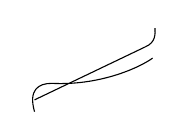
\begin{tikzpicture}[baseline=0cm,x=1cm,y=1cm]\draw[thin] (0,-.18)..controls (-.08,.1) and (.05,.18)..(.22,.18)..controls (.8,.15) and (1.3,.36)..(1.5,.5);\draw[thin] (0,-.03)--(1.4,.64)..controls (1.55,.7) and (1.53,.82)..(1.53,.88);\end{tikzpicture}}$\deleted{a}.G_{\deleted{\unsure{K|H}_a}\handwritten{K_\nu}}$ de $G_{K_{\deleted{a}\handwritten{\nu}}}$ ouvert d'indice $\deleted{a}\handwritten{\nu}$ (correspondant au sous-groupe des racines $\deleted{a}\handwritten{\nu}$.èmes de 1 dans le groupe des caractères $\handwritten{\overline}{\handwritten{\underline}{Q}}^{\handwritten{*}}$ de $G_{\handwritten{K_{\unsure{\deleted{a}\nu|\deleted{\alpha}\nu|\nu}}}}$)


